\documentclass[numbers=noenddot,10pt,a4paper]{scrartcl}
\usepackage[greek,ngerman]{babel}
\usepackage[T1]{fontenc}
\usepackage[utf8]{inputenc}
\usepackage{fullpage}
\usepackage{libertine}
\usepackage{ziffer}
\usepackage{graphicx}
\usepackage{units}
%\usepackage{wasysym}
\usepackage{amsmath}
\usepackage{amssymb}
\usepackage{wrapfig}
\usepackage{esint}
\usepackage{float}
\usepackage{wrapfig}
\usepackage[font=small]{caption}
\usepackage{subcaption}

\renewcommand{\thefigure}{Abb. \arabic{figure}}

\captionsetup[wrapfigure]{name=}
\captionsetup[figure]{name=}
\newcommand{\degree}{^\circ}
\newcommand{\diff}{\textnormal{d}}
\newcommand{\tenpo}[1]{\cdot 10^{#1}}
\newcommand{\greek}[1]{\greektext#1\latintext}
\newcommand{\ix}[1]{_\text{#1}}

\title{Protokoll: Schmitt-Trigger}
\author{Tom Kranz, Philipp Hacker}
\date{\today}

\begin{document}
%\setcounter{page}{2}
%\setcounter{section}{1}
\maketitle
\vspace*{\fill}
\tableofcontents
\vfill
\newpage
\section{Vorbereitung}
\subsection{Schaltskizzen}
\begin{figure}[H]
\centering
\begin{subfigure}[b]{0.49\textwidth}
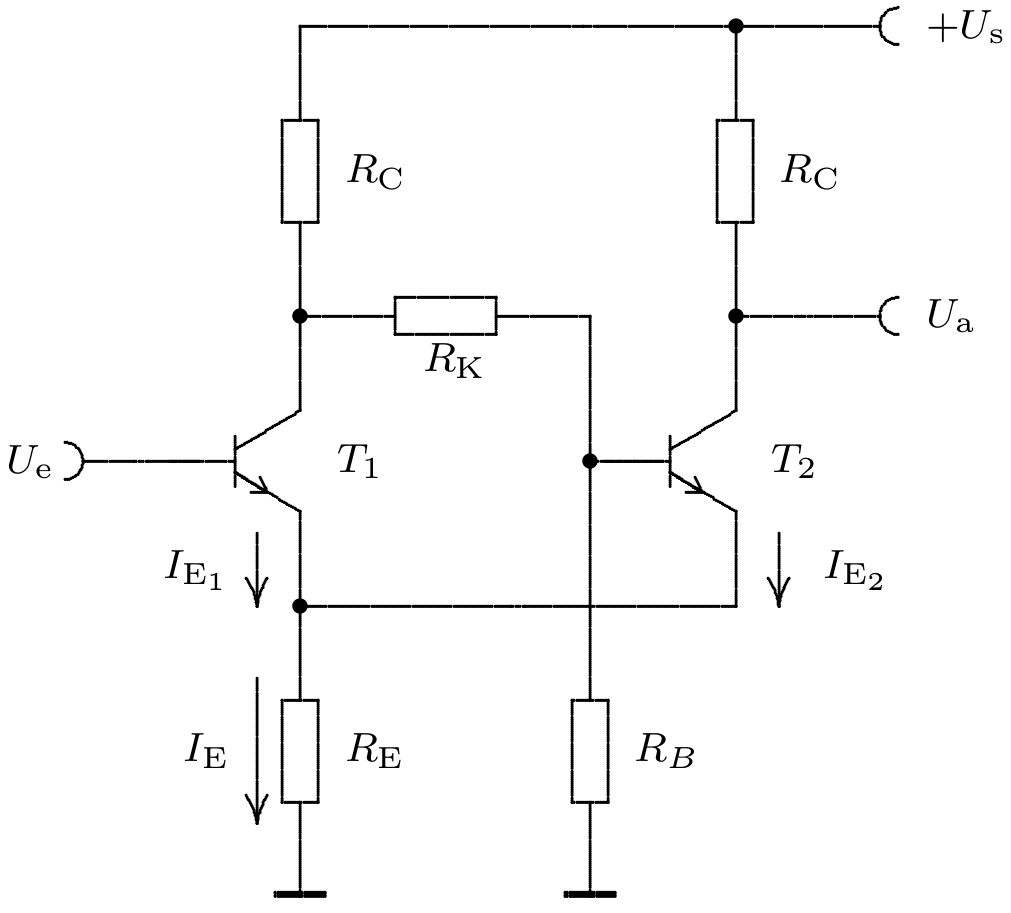
\includegraphics[width=\textwidth]{schaltskizze_st2.png}
\caption{Grundschaltung}
\end{subfigure}
\begin{subfigure}[b]{0.49\textwidth}
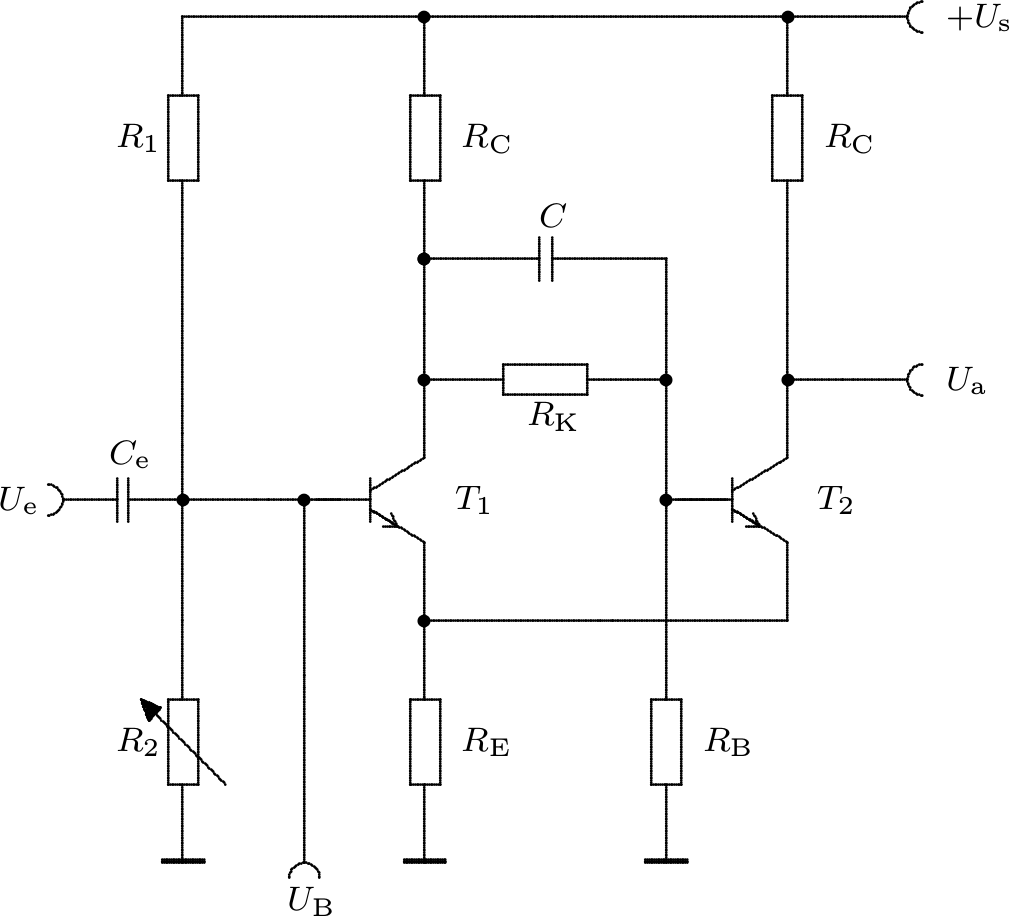
\includegraphics[width=\textwidth]{schaltskizze_st1.png}
\caption{Schaltung mit Modifizierungen $C$, $C\ix{e}$ sowie $R_1$ und $R_2$}
\end{subfigure}
\caption{Schaltbilder zum Schmitt-Trigger}
\end{figure}
\subsection{Dimensionierung}
\subsection{Vorbereitungsaufgaben 1 u. 2}
Schmitt-Trigger werden zur Erzeugung und Flankenversteilerung von Rechteckimpulsfolgen eingesetzt. Somit dienen sie meist der Umwandlung von analogen, beliebigen Signalen $U\ix{e}$ zu \textit{High-} und \textit{Lowpotentialen}, welche binär interpretiert werden können. Weiterhin nutzt man Schmitt-Trigger zur "`Entprellung"' von Schaltern (Auflösen des kurzzeitigen, mehrfachen Öffnens und Schließens eines Tasters) und der Schwingungserzeugung. \\
Die sogenannte Schalthysteresis ist die Differenz aus \textit{High-} und \textit{Low}zustand des ST (\textit{High-} u. \textit{Low}potential fallen nicht zusammen). Sie bestimmt wann das Eingangssignal $U\ix{e}$ als ein Ein- bzw. Ausschalten des Triggers interpretiert wird. Für eben dieses $\Delta U$ gilt näherungsweise
\begin{align}
\Delta U=U_+-U_-\approx\left(U\ix{E}-U\ix{BE;Schw}\right)-\left(U\ix{E}-U\ix{CE;sat}\right)=U\ix{BE;Schw}-U\ix{CE;sat}
\end{align}
\begin{figure}[H]
\centering
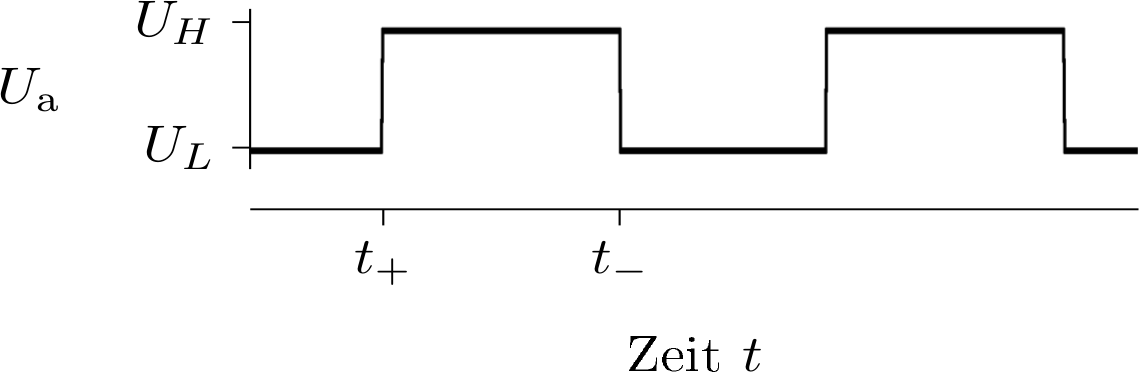
\includegraphics[width=0.55\textwidth]{ausgangssignal.png}
\caption{Ausgangssignal $U\ix{a}$ über $t$ (schematisch; ideal)}
\label{img:signal}
\end{figure}
Die Flankenversteilerung des Ausgangssignals des Schmitt-Triggers (\ref{img:signal}) kann dadurch erreicht werden, dass mittels eines Kondensators $R\ix{K}$ überbrückt wird. Dies hat zur Folge, dass die Spannungssprünge in den Zeitpunkten $t_+$ bzw. $t_-$ vom Kollektor von $T_1$ direkt auf die Basis von $T_2$ übertragen werden können.
\section{Durchführung}
\subsection{Messgeräte}
\subsection{Oszillogramme}
\section{Auswertung}
\section{Anhang}
Die originalen Messwert-Aufzeichnungen liegen bei.
\end{document}